% \newpage
\section{Dodawanie nowych zleceń}

Dodawanie nowych zleceń jest jedną z głównych funkcjonalności, która jest specyficzna dla klientów. Z tego powodu została umieszczona w ich aplikacji. Składa się na nią aż pięć ekranów, które przedstawiono na rysunku \ref{fig:add-job}. Każdy z nich stanowi inny etap procesu tworzenia zlecenia. Poruszanie pomiędzy nimi odbywa się sekwencyjnie - aby dostać się do danego ekranu trzeba przejść przez wszystkie wcześniejsze. 

Dodawanie zlecenia rozpoczyna się od zakładki \enquote{dodaj zlecenie} znajdującej się na ekranie głównym aplikacji dla klientów. Zawiera listę wszystkich dostępnych kategorii. Po wybraniu jednej z nich użytkownik zostaje przeniesiony do ekranu, który przedstawia podobną listę, lecz zawierającą usługi, które należą do wybranej chwilę wcześniej kategorii. Od tego momentu widoczny jest pasek postępu, który informuje o aktualnym etapie tworzenia zlecenia. Gdy usługa również zostanie wybrana, to bieżący widok zmienia się w ekran wyboru lokalizacji. Przy jego pomocy określane jest miejsce, w którym usługa ma być świadczona. Miejscowość można wpisać przy pomocy przeznaczonego do tego pola, które zapewnia automatyczne uzupełnienie. Spodziewano się jednak, że klienci często będą korzystali z tych samych lokalizacji. Może nią być na przykład miejsca zamieszkania. Z tego powodu przewidziano funkcję zapamiętywania tych ostatnio wprowadzonych i możliwość ich szybkiego wyboru z listy. Przenosi on użytkownika do ekranu uzupełnienia szczegółów. W przeznaczonym na to miejscu klienci mogą przedstawić szczegóły usługi, której wykonania wymagają, a w polu czasu realizacji określają żądany termin wykonania. Zamiast pola tekstowego rozważano możliwość wprowadzania tej informacji w sposób bardziej ścisły, na przykład poprzez wybranie konkretnych dni i godzin. Uznano jednak to rozwiązanie za zbyt ograniczające. W przypadku wartości tekstowej można bowiem użyć zwrotów bardziej ogólnych, takich jak: \enquote{jak najczybciej}, czy też \enquote{najlepiej przed}. Po uzupełnieniu obu pól i zatwierdzeniu zlecenie o podanych parametrach jest tworzone, a użytkownik zostaje o tym powiadomiony.

\begin{figure}[htp!]
  \captionsetup[subfigure]{justification=centering}
  \centering
  \begin{subfigure}[t]{0.32\textwidth}
    \centering
    \fbox{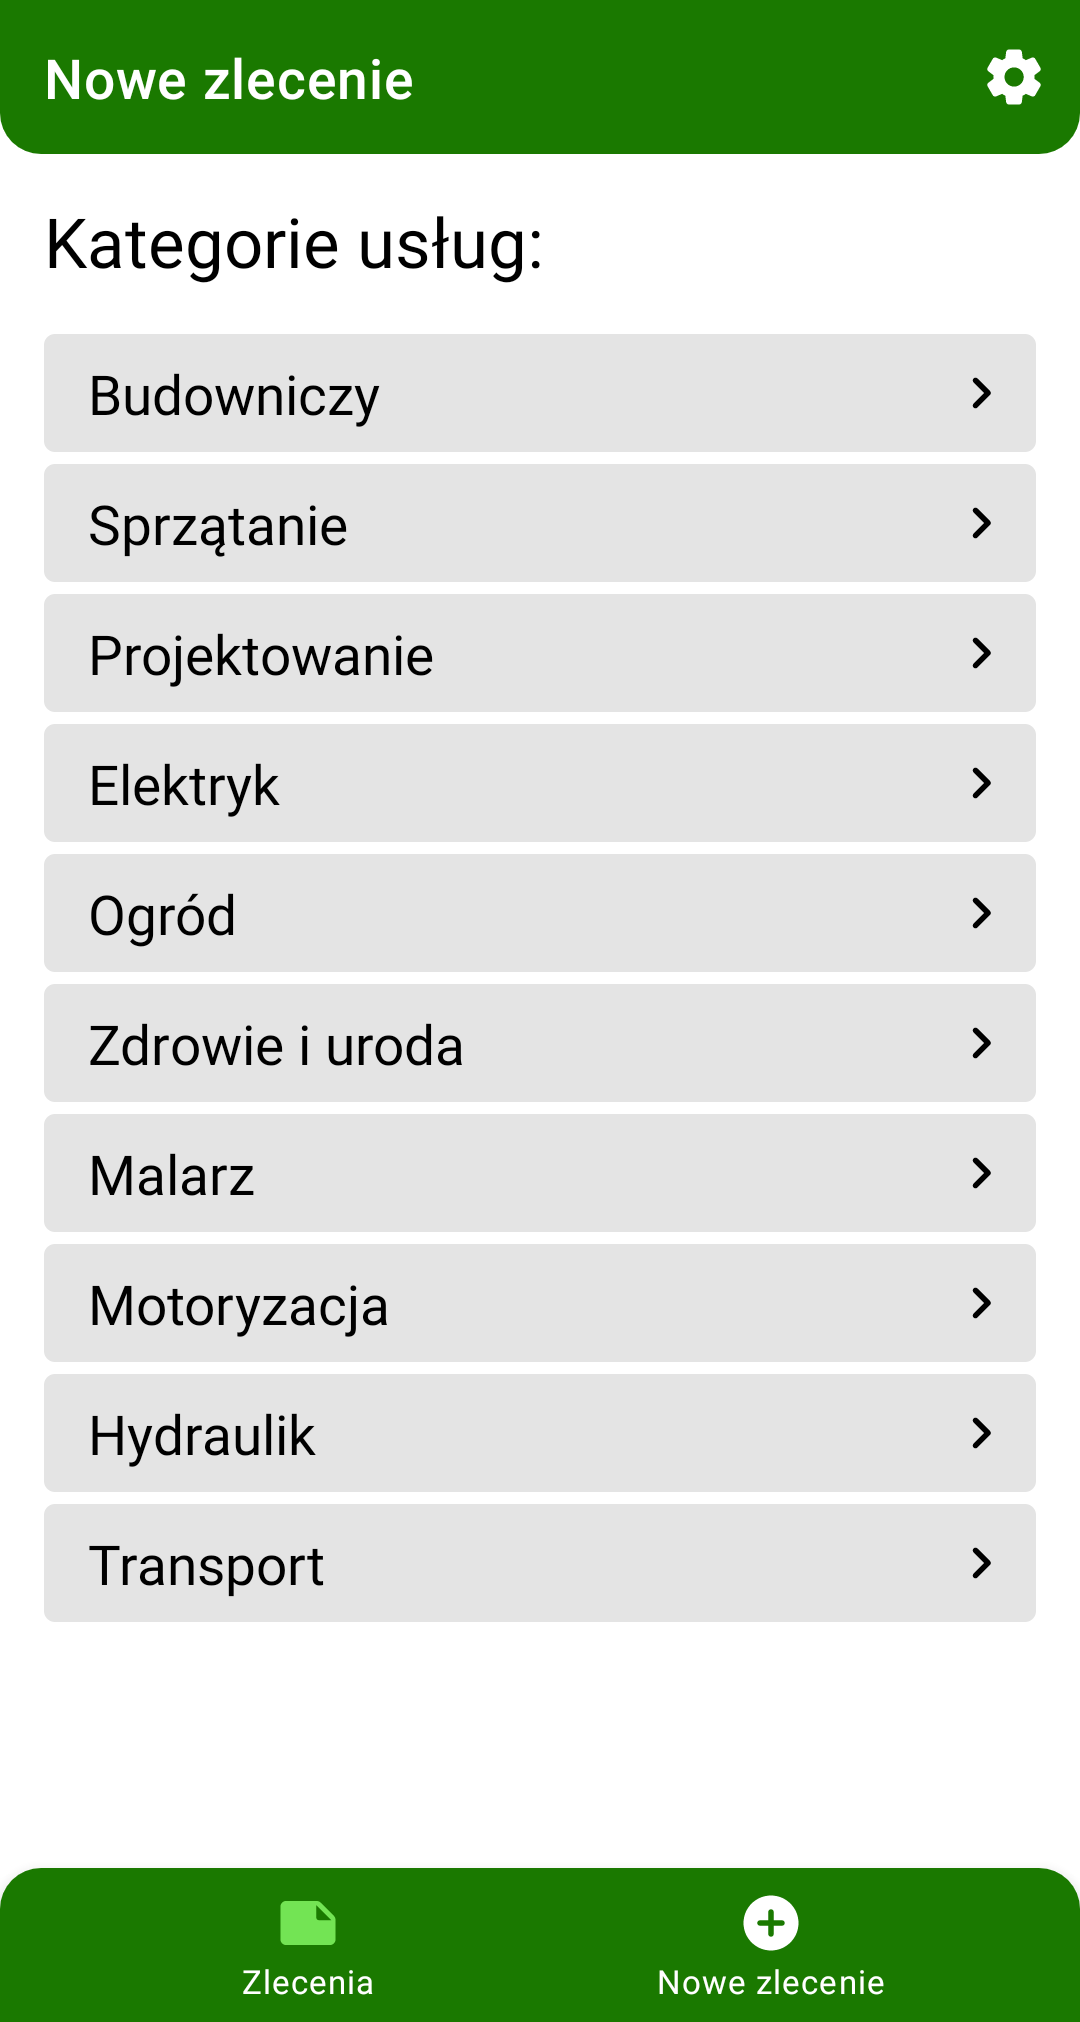
\includegraphics[width=0.97\linewidth]{screens/add_job_category.png}}
    \caption{Ekran wyboru kategorii}
  \end{subfigure}
  \begin{subfigure}[t]{0.32\textwidth}
    \centering
    \fbox{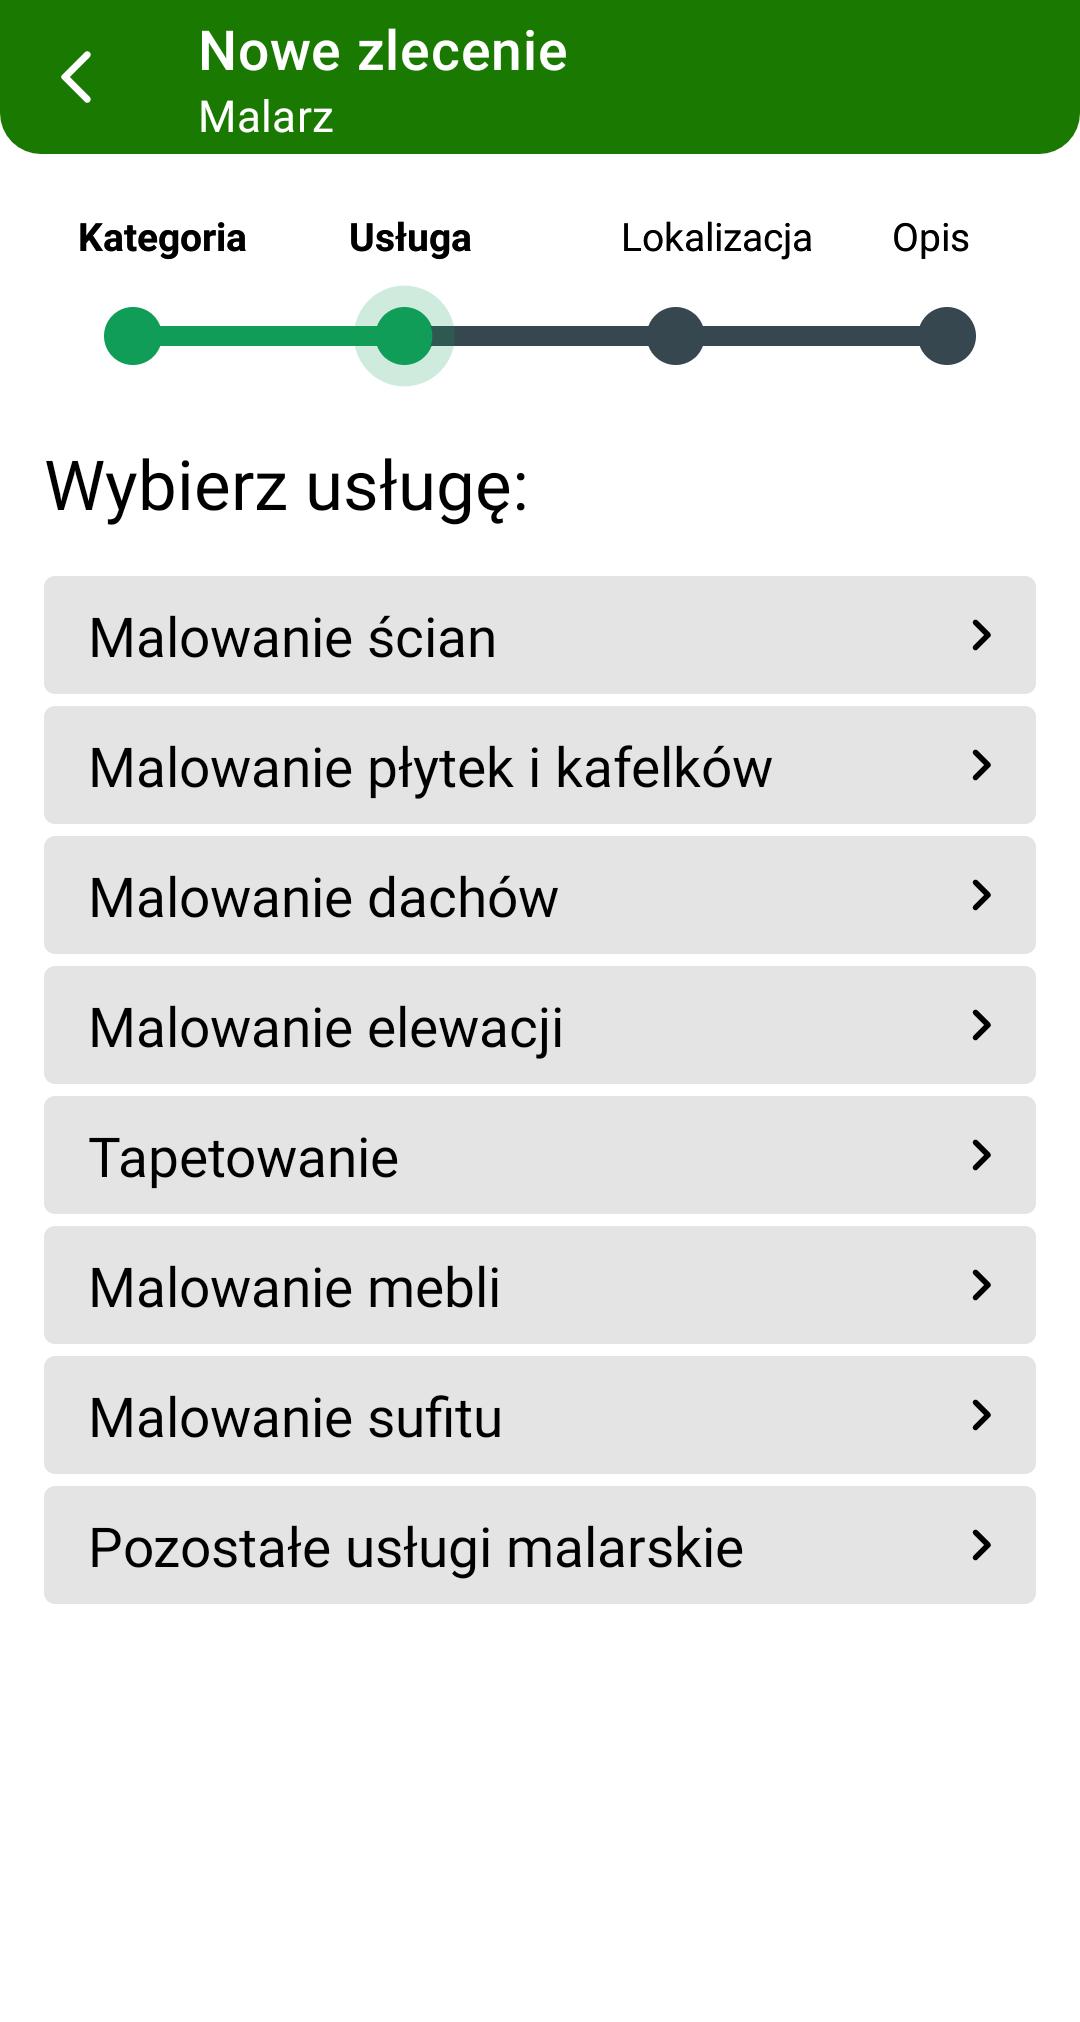
\includegraphics[width=0.97\linewidth]{screens/add_job_service.png}}
    \caption{Ekran wyboru usługi}
  \end{subfigure}
  \begin{subfigure}[t]{0.32\textwidth}
    \centering
    \fbox{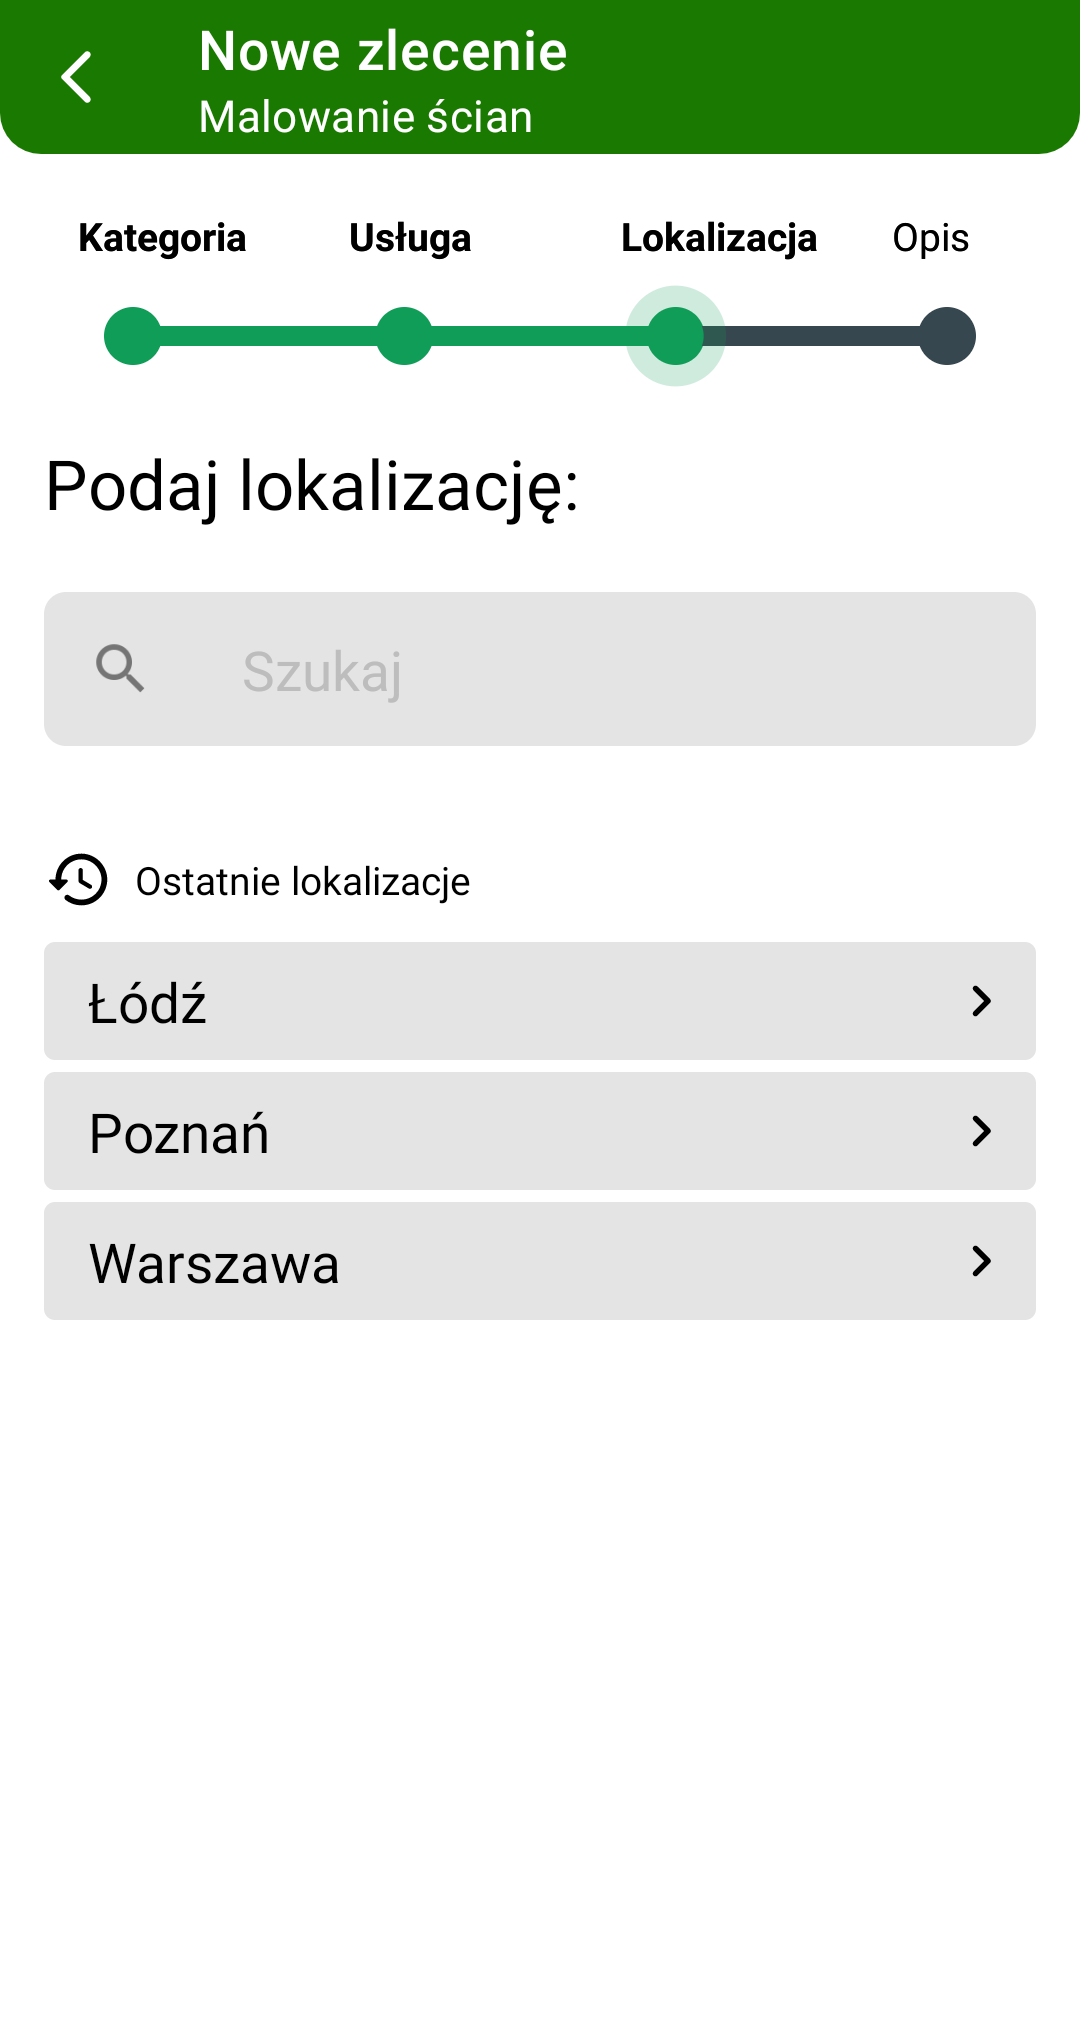
\includegraphics[width=0.97\linewidth]{screens/add_job_location.png}}
    \caption{Ekran wyboru lokalizacji}
  \end{subfigure}
  \vskip\baselineskip
  \vskip\baselineskip
  \vskip\baselineskip
  \begin{subfigure}[t]{0.32\textwidth}
    \centering
    \fbox{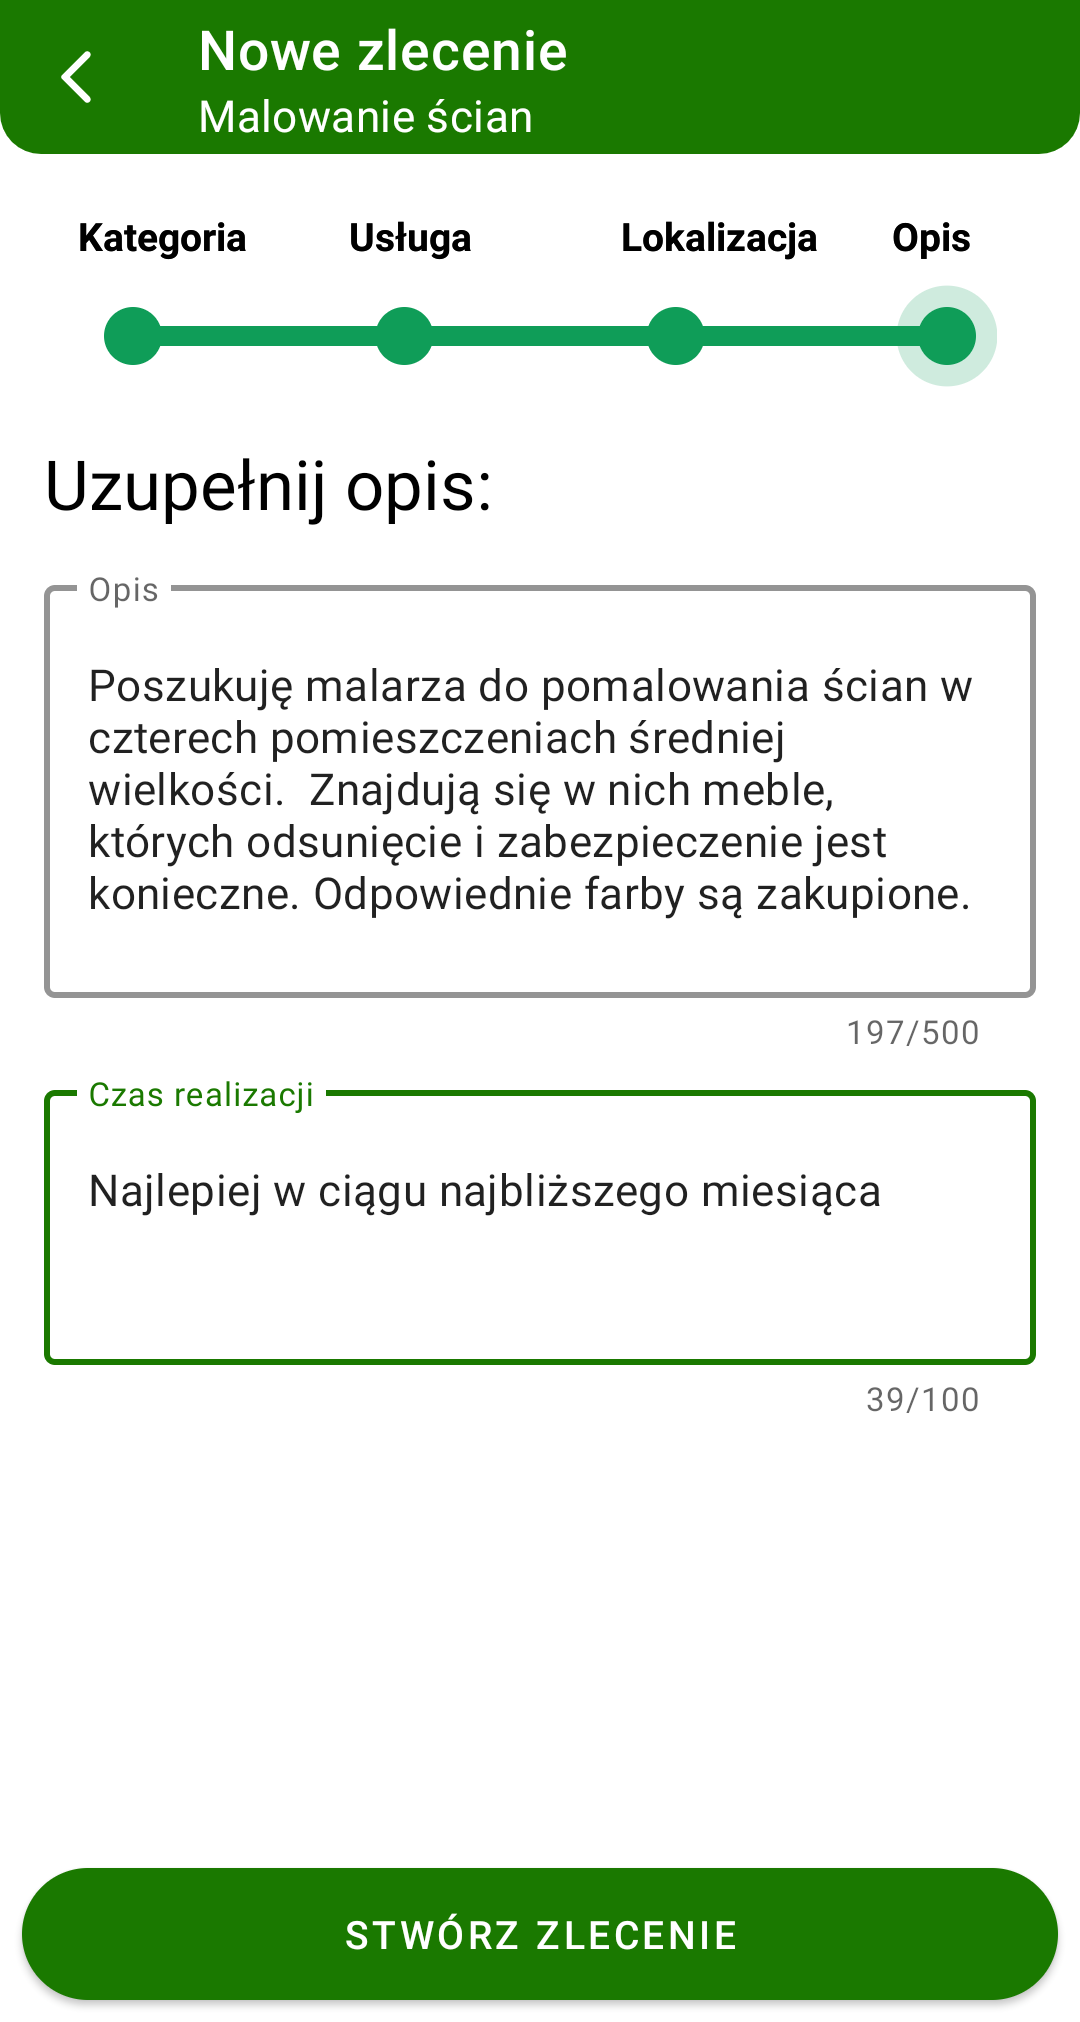
\includegraphics[width=0.97\linewidth]{screens/add_job_details.png}}
    \caption{Ekran uzupełnienia opisu}
  \end{subfigure}
  \begin{subfigure}[t]{0.32\textwidth}
    \centering
    \fbox{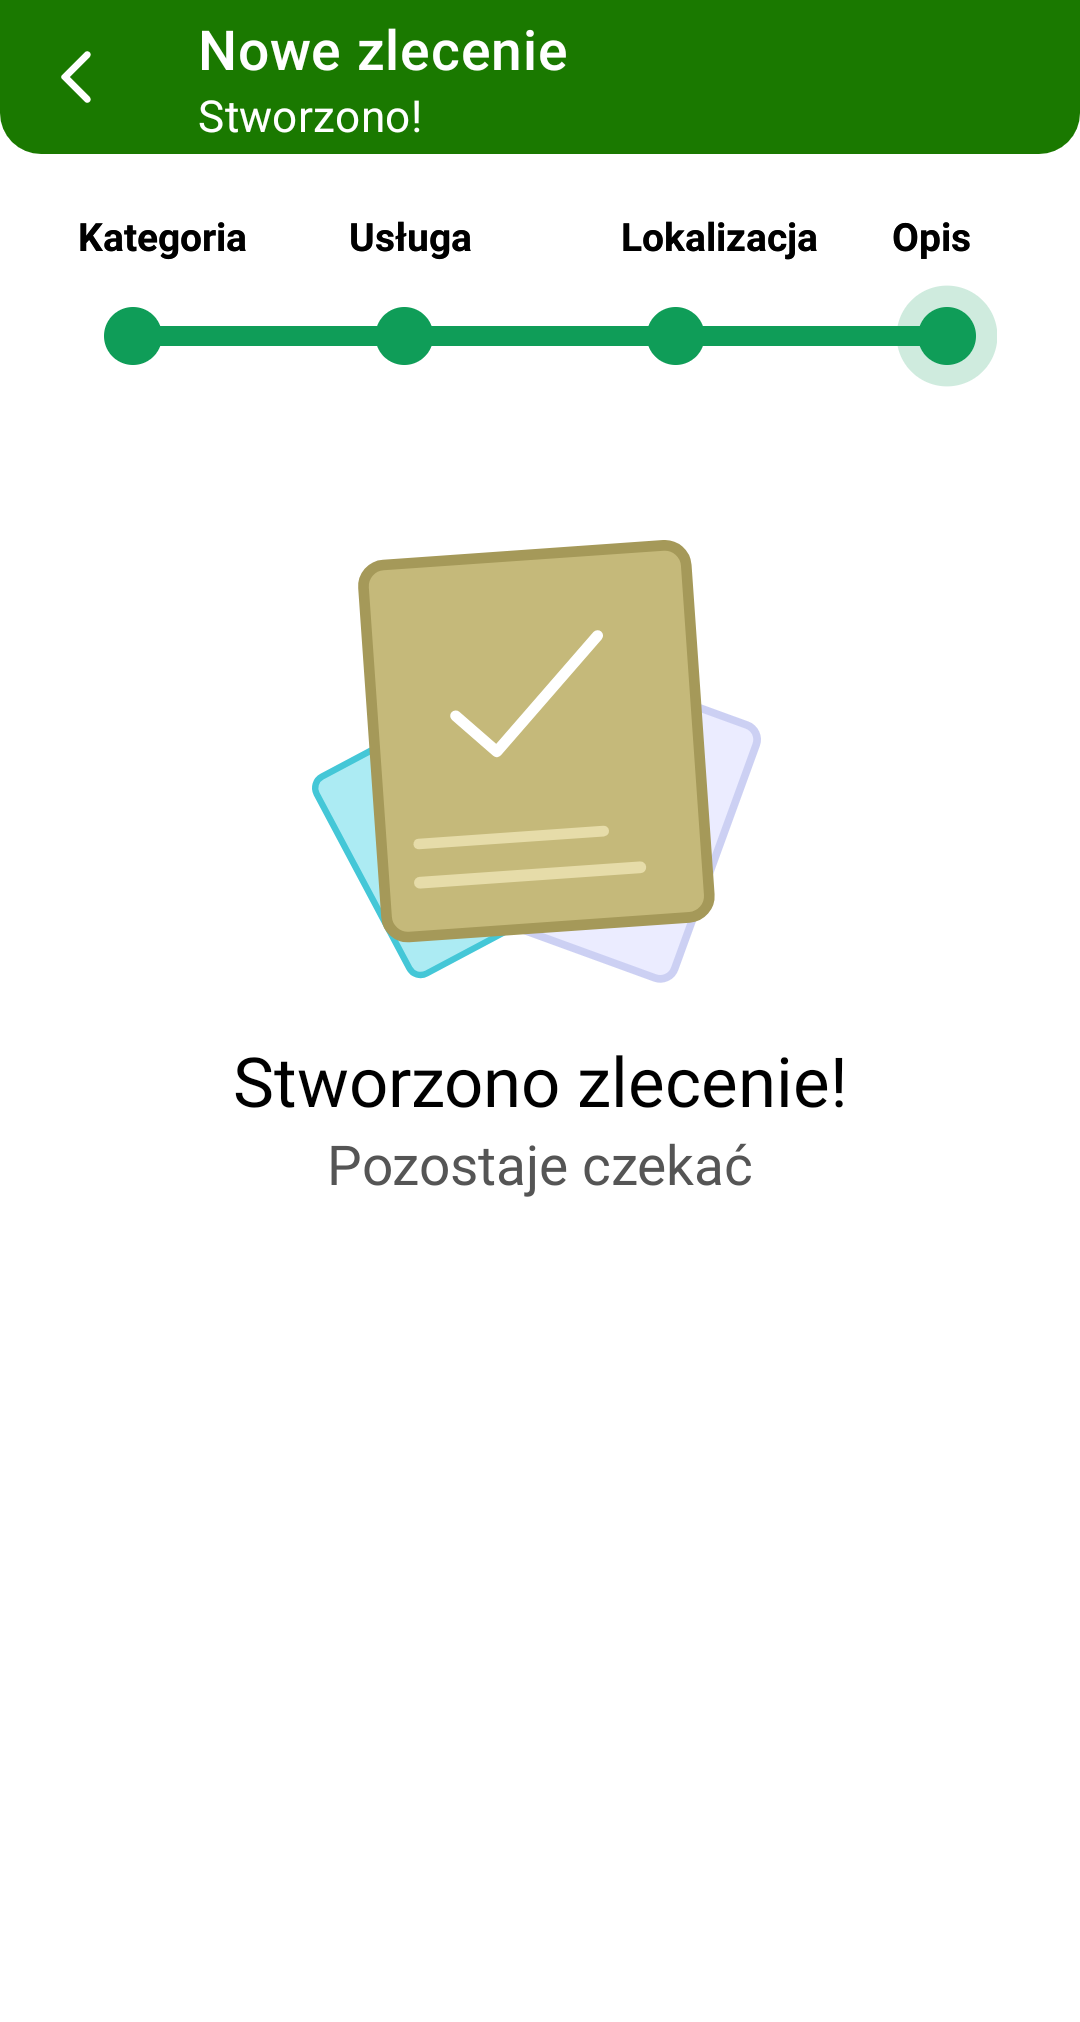
\includegraphics[width=0.97\linewidth]{screens/add_job_done.png}}
    \caption{Ekran potwierdzenia dodania}
  \end{subfigure}
  \caption{Ekrany dodawania zlecenia}
  \label{fig:add-job}
\end{figure}